% Created by tikzDevice version 0.12.6 on 2025-01-28 09:53:54
% !TEX encoding = UTF-8 Unicode
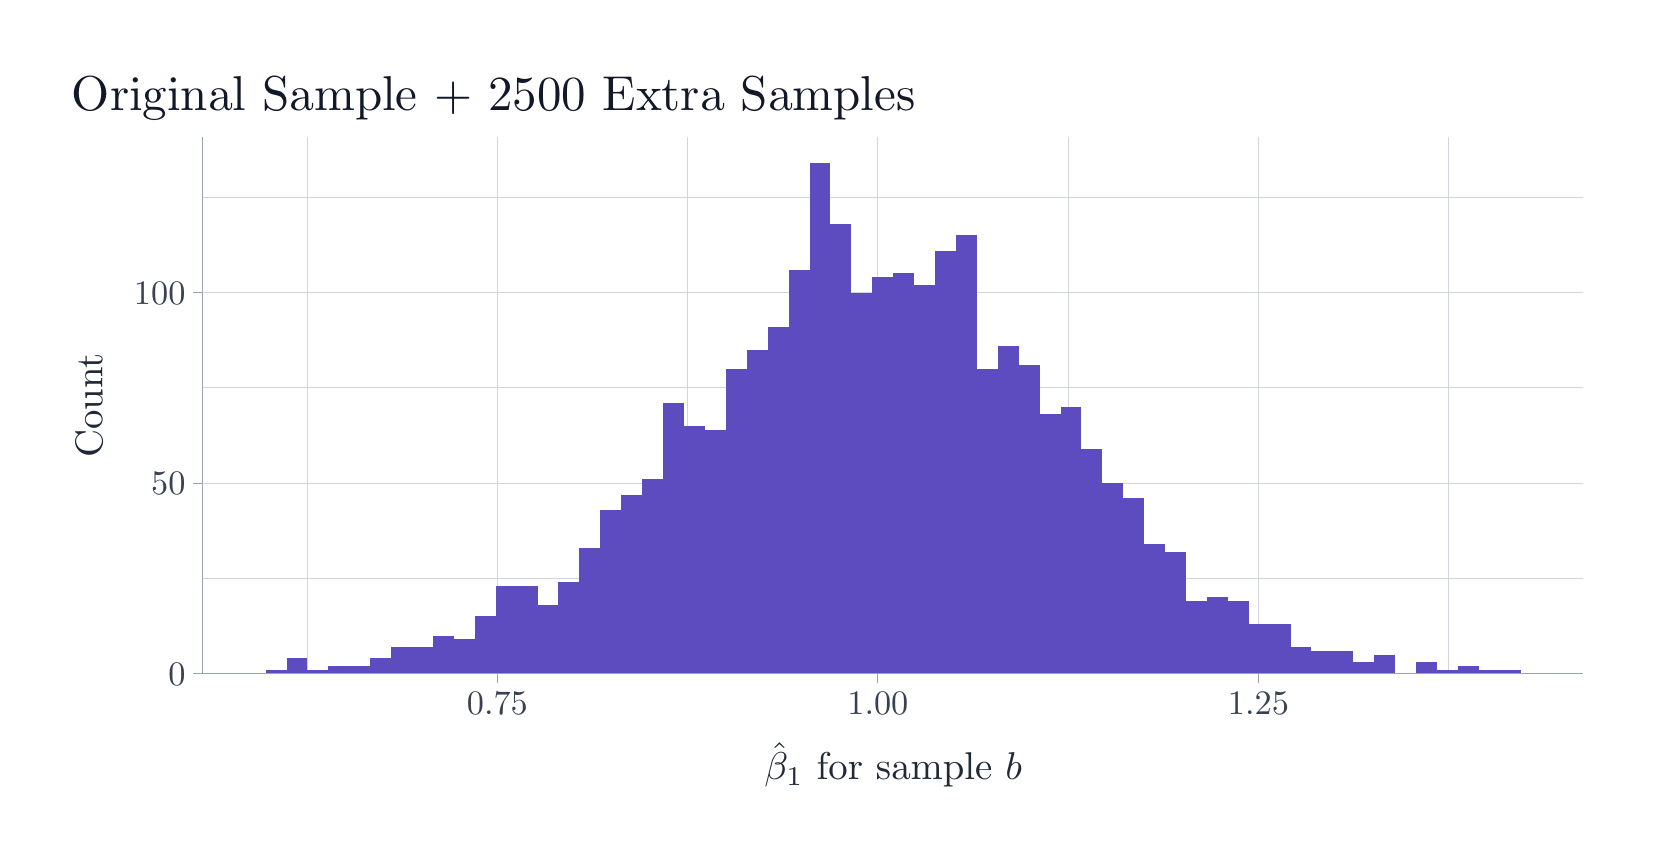
\begin{tikzpicture}[x=1pt,y=1pt]
\definecolor{fillColor}{RGB}{255,255,255}
\path[use as bounding box,fill=fillColor] (0,0) rectangle (578.16,289.08);
\begin{scope}
\path[clip] (  0.00,  0.00) rectangle (578.16,289.08);
\definecolor{drawColor}{RGB}{255,255,255}

\path[draw=drawColor,line width= 0.7pt,line join=round,line cap=round,fill=fillColor] (  0.00,  0.00) rectangle (578.16,289.08);
\end{scope}
\begin{scope}
\path[clip] ( 63.32, 55.65) rectangle (562.16,249.43);
\definecolor{drawColor}{RGB}{255,255,255}
\definecolor{fillColor}{RGB}{255,255,255}

\path[draw=drawColor,line width= 0.7pt,line join=round,line cap=round,fill=fillColor] ( 63.32, 55.65) rectangle (562.16,249.43);
\definecolor{drawColor}{RGB}{209,213,219}

\path[draw=drawColor,line width= 0.4pt,line join=round] ( 63.32, 90.08) --
	(562.16, 90.08);

\path[draw=drawColor,line width= 0.4pt,line join=round] ( 63.32,158.94) --
	(562.16,158.94);

\path[draw=drawColor,line width= 0.4pt,line join=round] ( 63.32,227.81) --
	(562.16,227.81);

\path[draw=drawColor,line width= 0.4pt,line join=round] (100.97, 55.65) --
	(100.97,249.43);

\path[draw=drawColor,line width= 0.4pt,line join=round] (238.47, 55.65) --
	(238.47,249.43);

\path[draw=drawColor,line width= 0.4pt,line join=round] (375.98, 55.65) --
	(375.98,249.43);

\path[draw=drawColor,line width= 0.4pt,line join=round] (513.48, 55.65) --
	(513.48,249.43);

\path[draw=drawColor,line width= 0.4pt,line join=round] ( 63.32, 55.65) --
	(562.16, 55.65);

\path[draw=drawColor,line width= 0.4pt,line join=round] ( 63.32,124.51) --
	(562.16,124.51);

\path[draw=drawColor,line width= 0.4pt,line join=round] ( 63.32,193.38) --
	(562.16,193.38);

\path[draw=drawColor,line width= 0.4pt,line join=round] (169.72, 55.65) --
	(169.72,249.43);

\path[draw=drawColor,line width= 0.4pt,line join=round] (307.23, 55.65) --
	(307.23,249.43);

\path[draw=drawColor,line width= 0.4pt,line join=round] (444.73, 55.65) --
	(444.73,249.43);
\definecolor{fillColor}{RGB}{92,76,191}

\path[fill=fillColor] ( 85.99, 55.65) rectangle ( 93.55, 57.03);

\path[fill=fillColor] ( 93.55, 55.65) rectangle (101.11, 61.16);

\path[fill=fillColor] (101.11, 55.65) rectangle (108.67, 57.03);

\path[fill=fillColor] (108.67, 55.65) rectangle (116.23, 58.40);

\path[fill=fillColor] (116.23, 55.65) rectangle (123.78, 58.40);

\path[fill=fillColor] (123.78, 55.65) rectangle (131.34, 61.16);

\path[fill=fillColor] (131.34, 55.65) rectangle (138.90, 65.29);

\path[fill=fillColor] (138.90, 55.65) rectangle (146.46, 65.29);

\path[fill=fillColor] (146.46, 55.65) rectangle (154.02, 69.42);

\path[fill=fillColor] (154.02, 55.65) rectangle (161.58, 68.04);

\path[fill=fillColor] (161.58, 55.65) rectangle (169.13, 76.31);

\path[fill=fillColor] (169.13, 55.65) rectangle (176.69, 87.33);

\path[fill=fillColor] (176.69, 55.65) rectangle (184.25, 87.33);

\path[fill=fillColor] (184.25, 55.65) rectangle (191.81, 80.44);

\path[fill=fillColor] (191.81, 55.65) rectangle (199.37, 88.70);

\path[fill=fillColor] (199.37, 55.65) rectangle (206.92,101.10);

\path[fill=fillColor] (206.92, 55.65) rectangle (214.48,114.87);

\path[fill=fillColor] (214.48, 55.65) rectangle (222.04,120.38);

\path[fill=fillColor] (222.04, 55.65) rectangle (229.60,125.89);

\path[fill=fillColor] (229.60, 55.65) rectangle (237.16,153.44);

\path[fill=fillColor] (237.16, 55.65) rectangle (244.72,145.17);

\path[fill=fillColor] (244.72, 55.65) rectangle (252.27,143.79);

\path[fill=fillColor] (252.27, 55.65) rectangle (259.83,165.83);

\path[fill=fillColor] (259.83, 55.65) rectangle (267.39,172.72);

\path[fill=fillColor] (267.39, 55.65) rectangle (274.95,180.98);

\path[fill=fillColor] (274.95, 55.65) rectangle (282.51,201.64);

\path[fill=fillColor] (282.51, 55.65) rectangle (290.06,240.20);

\path[fill=fillColor] (290.06, 55.65) rectangle (297.62,218.17);

\path[fill=fillColor] (297.62, 55.65) rectangle (305.18,193.38);

\path[fill=fillColor] (305.18, 55.65) rectangle (312.74,198.89);

\path[fill=fillColor] (312.74, 55.65) rectangle (320.30,200.26);

\path[fill=fillColor] (320.30, 55.65) rectangle (327.86,196.13);

\path[fill=fillColor] (327.86, 55.65) rectangle (335.41,208.53);

\path[fill=fillColor] (335.41, 55.65) rectangle (342.97,214.04);

\path[fill=fillColor] (342.97, 55.65) rectangle (350.53,165.83);

\path[fill=fillColor] (350.53, 55.65) rectangle (358.09,174.09);

\path[fill=fillColor] (358.09, 55.65) rectangle (365.65,167.21);

\path[fill=fillColor] (365.65, 55.65) rectangle (373.21,149.30);

\path[fill=fillColor] (373.21, 55.65) rectangle (380.76,152.06);

\path[fill=fillColor] (380.76, 55.65) rectangle (388.32,136.91);

\path[fill=fillColor] (388.32, 55.65) rectangle (395.88,124.51);

\path[fill=fillColor] (395.88, 55.65) rectangle (403.44,119.00);

\path[fill=fillColor] (403.44, 55.65) rectangle (411.00,102.48);

\path[fill=fillColor] (411.00, 55.65) rectangle (418.55, 99.72);

\path[fill=fillColor] (418.55, 55.65) rectangle (426.11, 81.82);

\path[fill=fillColor] (426.11, 55.65) rectangle (433.67, 83.19);

\path[fill=fillColor] (433.67, 55.65) rectangle (441.23, 81.82);

\path[fill=fillColor] (441.23, 55.65) rectangle (448.79, 73.55);

\path[fill=fillColor] (448.79, 55.65) rectangle (456.35, 73.55);

\path[fill=fillColor] (456.35, 55.65) rectangle (463.90, 65.29);

\path[fill=fillColor] (463.90, 55.65) rectangle (471.46, 63.91);

\path[fill=fillColor] (471.46, 55.65) rectangle (479.02, 63.91);

\path[fill=fillColor] (479.02, 55.65) rectangle (486.58, 59.78);

\path[fill=fillColor] (486.58, 55.65) rectangle (494.14, 62.54);

\path[fill=fillColor] (494.14, 55.65) rectangle (501.69, 55.65);

\path[fill=fillColor] (501.69, 55.65) rectangle (509.25, 59.78);

\path[fill=fillColor] (509.25, 55.65) rectangle (516.81, 57.03);

\path[fill=fillColor] (516.81, 55.65) rectangle (524.37, 58.40);

\path[fill=fillColor] (524.37, 55.65) rectangle (531.93, 57.03);

\path[fill=fillColor] (531.93, 55.65) rectangle (539.49, 57.03);
\end{scope}
\begin{scope}
\path[clip] (  0.00,  0.00) rectangle (578.16,289.08);
\definecolor{drawColor}{RGB}{156,163,175}

\path[draw=drawColor,line width= 0.3pt,line join=round] ( 63.32, 55.65) --
	( 63.32,249.43);
\end{scope}
\begin{scope}
\path[clip] (  0.00,  0.00) rectangle (578.16,289.08);
\definecolor{drawColor}{RGB}{55,65,81}

\node[text=drawColor,anchor=base east,inner sep=0pt, outer sep=0pt, scale=  1.24] at ( 57.02, 51.37) {0};

\node[text=drawColor,anchor=base east,inner sep=0pt, outer sep=0pt, scale=  1.24] at ( 57.02,120.23) {50};

\node[text=drawColor,anchor=base east,inner sep=0pt, outer sep=0pt, scale=  1.24] at ( 57.02,189.09) {100};
\end{scope}
\begin{scope}
\path[clip] (  0.00,  0.00) rectangle (578.16,289.08);
\definecolor{drawColor}{RGB}{156,163,175}

\path[draw=drawColor,line width= 0.3pt,line join=round] ( 59.82, 55.65) --
	( 63.32, 55.65);

\path[draw=drawColor,line width= 0.3pt,line join=round] ( 59.82,124.51) --
	( 63.32,124.51);

\path[draw=drawColor,line width= 0.3pt,line join=round] ( 59.82,193.38) --
	( 63.32,193.38);
\end{scope}
\begin{scope}
\path[clip] (  0.00,  0.00) rectangle (578.16,289.08);
\definecolor{drawColor}{RGB}{156,163,175}

\path[draw=drawColor,line width= 0.3pt,line join=round] ( 63.32, 55.65) --
	(562.16, 55.65);
\end{scope}
\begin{scope}
\path[clip] (  0.00,  0.00) rectangle (578.16,289.08);
\definecolor{drawColor}{RGB}{156,163,175}

\path[draw=drawColor,line width= 0.3pt,line join=round] (169.72, 52.15) --
	(169.72, 55.65);

\path[draw=drawColor,line width= 0.3pt,line join=round] (307.23, 52.15) --
	(307.23, 55.65);

\path[draw=drawColor,line width= 0.3pt,line join=round] (444.73, 52.15) --
	(444.73, 55.65);
\end{scope}
\begin{scope}
\path[clip] (  0.00,  0.00) rectangle (578.16,289.08);
\definecolor{drawColor}{RGB}{55,65,81}

\node[text=drawColor,anchor=base,inner sep=0pt, outer sep=0pt, scale=  1.24] at (169.72, 40.78) {0.75};

\node[text=drawColor,anchor=base,inner sep=0pt, outer sep=0pt, scale=  1.24] at (307.23, 40.78) {1.00};

\node[text=drawColor,anchor=base,inner sep=0pt, outer sep=0pt, scale=  1.24] at (444.73, 40.78) {1.25};
\end{scope}
\begin{scope}
\path[clip] (  0.00,  0.00) rectangle (578.16,289.08);
\definecolor{drawColor}{RGB}{31,41,55}

\node[text=drawColor,anchor=base,inner sep=0pt, outer sep=0pt, scale=  1.40] at (312.74, 17.36) {$\hat{\beta}_1$ for sample $b$};
\end{scope}
\begin{scope}
\path[clip] (  0.00,  0.00) rectangle (578.16,289.08);
\definecolor{drawColor}{RGB}{31,41,55}

\node[text=drawColor,rotate= 90.00,anchor=base,inner sep=0pt, outer sep=0pt, scale=  1.40] at ( 27.00,152.54) {Count};
\end{scope}
\begin{scope}
\path[clip] (  0.00,  0.00) rectangle (578.16,289.08);
\definecolor{drawColor}{RGB}{17,24,39}

\node[text=drawColor,anchor=base west,inner sep=0pt, outer sep=0pt, scale=  1.77] at ( 16.00,259.15) {Original Sample + 2500 Extra Samples};
\end{scope}
\end{tikzpicture}
